\newpage
\ifthenelse {\boolean{bachelor}}
{
	%\section{Analysis}
	\section{Matematické základy}\label{sec:matematicke_zaklady}
}
{
	%\chapter{Analysis}
%	\chapter{Analyza}
}

Tu začíname doplnat text. Ked chcete skompilovat ctrl+s a skomplilujete main.tex nekompilujte tento subor. Také zakladné pravidlá aby sme sa vedeli orientovať obrázky davajte do priečinka figures. Ak budete chciet robit referenciu na obrazok, rovnicu alebo sekcie : \ref{sec:matematicke_zaklady}. Preto prosím každý obrázok, sekciu a rovnicu label-ujte, ulahci to robotu. Ja mam vo zvyku sekcie nazyvat sec:nazov, obrazky fig:nazov, rovnice eq:nazov. 

\newpage
\section{Metóda spätnoväzobnej linearizácie}
tu by mohla byt nejaka teoria o spätnoväzobnej linearizácií
\newpage
\section{Vstupno-stavová metóda spätnoväzobnej linearizácie}
tu by mohla byt nejaka teoria o spätnoväzobnej linearizácií VS
\subsection{Návrh riadenia - Príklad 1.}
tu bude priklad 1 + vypocet
\subsection{Simulačná schéma - Príklad 1.}
tu schema 
\subsection{Overenie navrhnutého riadenia - Príklad 1.}
tu vysledky co sme dosiahli plus nejaky pokec k tomu
\subsection{Návrh riadenia - Príklad 2.}
\subsection{Simulačná schéma - Príklad 2.}
\subsection{Overenie navrhnutého riadenia - Príklad 2.}
\subsection{Porovnanie navrhnutého riadenia s lineárnym regulátorom}

\newpage
\section{Vstupno-výstupná metóda spätnoväzobnej linearizácie}
\subsection{Návrh riadenia - Príklad 1.}
\subsection{Simulačná schéma - Príklad 1.}
\subsection{Overenie navrhnutého riadenia - Príklad 1.}
\subsection{Návrh riadenia - Príklad 2.}
\subsection{Simulačná schéma - Príklad 2.}
\subsection{Overenie navrhnutého riadenia - Príklad 2.}
\subsection{Porovnanie navrhnutého riadenia s lineárnym regulátorom}



\newpage
\section{Prehlad takych zakladnych latex veci - Tato sekcia tu nebude }\label{sec:prehlad}

$ H = \begin{bmatrix} 18.9000 & 47.6000 & 63.0000 \\ 28.7000 & 44.1000 & 45.5000 \\ 15.4000  & 16.8000  & 12.6000 \\ 1.4000 & -2.8000  & -7.0000 \end{bmatrix}$
$ y = \begin{bmatrix} -64.4000 \\ -41.3000 \\ -8.4000 \\ 8.4000 \end{bmatrix}$

\begin{equation}\label{eq:Rovnica}
F(s) = \frac{K}{1+Ts}e^{-Ds}
\end{equation}


\textbf{Neznáme parametre:} $K,T,D$


\textbf{Postup:}
\begin{enumerate}
\item \[K = y(\infty); K = 3.8059\]
\item \[T = \frac{t_2-t_1}{ln(\frac{K-y_1}{K-y_2})} ; T = 0.4452 \]
\item \[x = \frac{ln(\frac{K-y_1}{K})}{ln\frac{K-y_2}{K}}, D = \frac{t_2x-t_1}{x-1}; x = 0.2093, D = 0.0857\]
\end{enumerate}

\textbf{Postup:}
\begin{itemize}
\item \[K = y(\infty); K = 3.8059\]
\item \[T = \frac{t_2-t_1}{ln(\frac{K-y_1}{K-y_2})} ; T = 0.4452 \]
\item \[x = \frac{ln(\frac{K-y_1}{K})}{ln\frac{K-y_2}{K}}, D = \frac{t_2x-t_1}{x-1}; x = 0.2093, D = 0.0857\]
\end{itemize}

\begin{table}[h!]
\centering
 \begin{tabular}{|c | c | c | c | c|} 
 \hline
 $k$ & $\theta_{k}^{*}$ & $P_{k}$ & $e_{k}$ &  $Q_{k}$ \\ [0.5ex] 
 \hline\hline
 0 & $ \begin{bmatrix} 0 \\ 0 \\ 0 \end{bmatrix}$ & $ 10^{10} *\begin{bmatrix}  1 & 0 & 0 \\ 0 & 1 & 0 \\ 0 & 0  & 1 \end{bmatrix}$ & 0 & 0 \\ 
 \hline
 1 & $ \begin{bmatrix} -0.1846 \\ -0.4650 \\ -0.6155 \end{bmatrix}$ & $ 10^{9} *\begin{bmatrix}  9.4581 & -1.3648 & -1.8063 \\ -1.3648 & 6.5628 & -4.5492 \\ -1.8063  & -4.5492  & 3.9790 \end{bmatrix}$ & -64.4000 & $6.2915*10^{-11}$ \\ 
 \hline
 2 & $ \begin{bmatrix} 0.4987 \\ -0.2360 \\ -0.9935 \end{bmatrix}$ & $ 10^{9} *\begin{bmatrix}  2.4082 & -3.7279 & 2.0942 \\ -3.7279 & 5.7707 & -3.2418 \\ 2.0942 & -3.2418  & 1.8211 \end{bmatrix}$ & 12.5111 & $1.2915*10^{-10}$ \\ 
 \hline
 3 & $ \begin{bmatrix} 1.6486 \\ -2.0160\\ 0.0064 \end{bmatrix}$ & $\begin{bmatrix}  13.6362 & -21.4003 & 12.0936 \\ -21.4002 & 33.5946 & -18.9875 \\ 12.0935 & -18.9874  & 10.7325 \end{bmatrix}$ & 0.4031 & $6.7820*10^{-10}$ \\ 
  \hline
 4 & $ \begin{bmatrix} 0.8406 \\ -0.7436 \\ -0.7140 \end{bmatrix}$ & $\begin{bmatrix}  4.3694 & -6.8073 & 3.8314 \\ -6.8066 & 10.6133 & -5.9761 \\ 3.8311 & -5.9762  & 3.3659 \end{bmatrix}$ & 0.4920 & 0.0704 \\ [1ex] 

 \hline
 \end{tabular}
\end{table}

\begin{figure}[H]
\begin{center}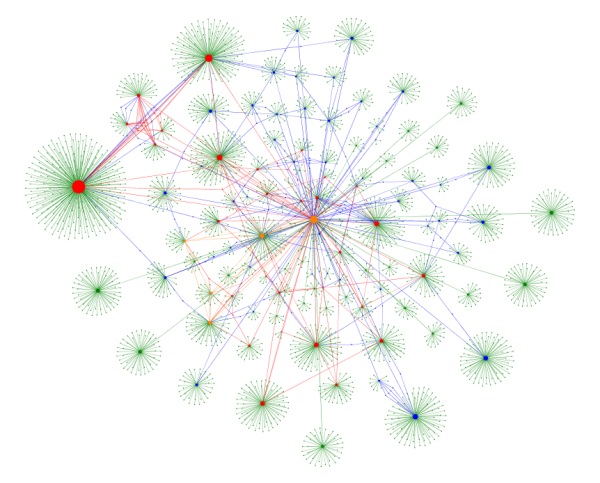
\includegraphics[scale=0.48]{figure.png}\end{center}
\caption{Name figure}\label{fig:figure}
\end{figure}
\subsection{Enumeration}
%\subsection{Číslovaný zoznam}
\begin{my_enumerate}
	\item {goal 1}
	\begin{my_enumerate}
		\item {goal 1.a}
		\item {goal 1.b}
	\end{my_enumerate}
	\item {goal 2}
	\item {goal 3}
\end{my_enumerate}
\subsection{Itemization}
%\subsection{Zoznam}
\begin{my_itemize}
	\item {item 1}
	\begin{my_itemize}
		\item {item 1.1}
		\item {item 1.2}
	\end{my_itemize}
	\item {item 2}
	\item {item 3}
\end{my_itemize}








